\section{Comportamento del Sistema}

\subsection{Descrizione della Rete di Petri}
Sfruttando i principi della programmazione reattiva, è possibile ottenere una versione sostanzialmente dichiarativa del sistema, dove la concorrenza è gestita tramite meccanismi interni della tecnologia utilizzata (RxJava, per l'appunto).\newline

\noindent Rispetto alla rete di Petri ottenuta precedentemente (\textit{vedi punto \ref{PN-part1}}), questa modellazione risulta molto più semplice e lineare; il sistema viene rappresentato da un flusso di eventi che si propagano in avanti e la cui computazione viene svolta in modo asincrono fino ad ottenere un risultato finale costruito sfruttando tutti i risultati parziali ottenuti fino a quel momento.\newline

\begin{figure}[H]
    \caption{Rete di Petri del sistema utilizzando la programmazione reattiva}
    \centering
    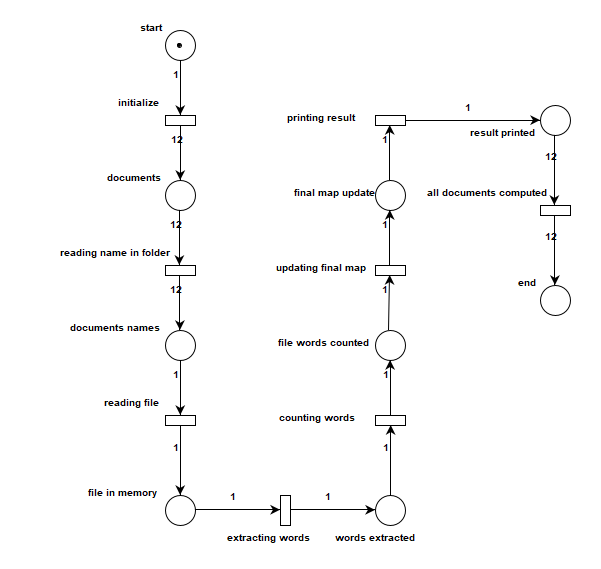
\includegraphics[width=120mm]{img/Petri net - Reactive Programming.png}
\end{figure}

\subsection{Approccio utilizzato}

\noindent Nella programmazione reattiva, sono possibili due approcci per la gestione degli Observable:
\begin{itemize}
    \item \textbf{Cold}\newline
    Nell'approccio Cold la propagazione di eventi inizia nel momento in cui vi è almeno un subscriber. Viene usato un modello \textbf{pull}, in quanto uno step successivo nel processo di elaborazione sarà eseguito solo nel momento in cui esista un risultato disponibile durante nello step immediatamente precedente nel flusso componente la computazione (la propagazione avviene dunque in modalità \textit{lazy}).
    \item \textbf{Hot}\newline
    Nell'approccio Hot la propagazione di eventi avviene continuamente e in modo indipendente dalla sottoscrizione di un observer. Questo modello viene dunque chiamato \textbf{push} e richiede la necessità di impiegare tecniche di backpressure per gestire casi in cui l'observer non riesce a consumare dati ad una velocità sufficiente a sostenere il ritmo con cui essi vengono prodotti.
\end{itemize}

\noindent Nel nostro caso è stato utilizzato un approccio cold. La nostra computazione difatti è dipendente dall'input dell'utente che, tramite l'interazione con un bottone, vi stabilirà un inizio (andando a sottoscrivere un Observer).\newline

\subsection{Utilizzo di RxJava}

\begin{minted}{java}
//used to define the behavior of onNext, onError and onComplete in subscribe
ComputationObserver computationObserver =
    ComputationObserver.createInstance(result, chrono);
//saving the disposable to use it in stopComputation
disposable = Observable
        .fromIterable(fileSystem.getPdfNames())
        .flatMap(pdf ->
                /*actual elaboration of a pdf, scheduled on a scheduler
                that uses the number of available processors*/
                Observable.just(pdf)
                        .subscribeOn(Schedulers.computation())
                        .map(fileSystem::createNewFileInstance)
                        .map(pdfElaboration::stringifyFile)
                        .map(pdfElaboration::createMapFromPDFString))
        .subscribe(
                computationObserver.getOnNextConsumer(),    //onNext
                computationObserver.getOnErrorConsumer(),   //onError
                computationObserver.getOnCompleteAction()   //onComplete
        );
\end{minted}

\noindent Il codice realizza, tramite RxJava, il comportamento descritto nella rete di Petri.\newline

\noindent Tale codice viene lanciato nel momento in in cui l'utente interagisce con l'apposito  bottone e, al fine di preservare la reattività della GUI, la subscribe utilizzata è di tipo non bloccante (in altri contesti sarebbe possibile, ad esempio, lanciare una \textit{blockingSubscribe}, la quale blocca l'esecuzione del thread chiamante fino al completamento della computazione eseguita nell'Observable). \newline

\noindent In RxJava la sottoscrizione ad un Observable produce un \textit{Disposable} e, attraverso di esso, è possibile interrompere prematuramente la computazione.

\begin{minted}{java}
disposable.dispose();
\end{minted}

\noindent L'Observable utilizza come fonte il set di nomi dei documenti PDF e, per ciascuno di essi, esegue concorrentemente gli step computazionali utilizzando l'approccio Cold descritto al punto \textit{3.3.2}.\newline

\noindent Ogniqualvolta venga completata l'elaborazione di un PDF, verrà eseguito quanto specificato nel Consumer onNext (in questo caso verrà aggiornata la UI stampando la situazione corrente del conteggio finale delle parole).\newline
\noindent Al termine dell'elaborazione di tutti i PDF verrà lanciata la Action onComplete (avvertendo l'utente della fine della computazione dei documenti).\newline
\noindent Nel caso ci fossero errori invece, verrà lanciato il Consume onError.
